% !TeX root = ../main.tex
% -*- coding: utf-8 -*-


\chapter{技术背景} 
\label{2}

本文的私有近边界数据主要是在近边界对抗性样本的基础上通过生成对抗网络生成的。本章首先介绍了深度神经网络的基本结构和知识产权保护领域相关术语,然后着重介绍了对抗性攻击和生成对抗网络的原理,为\ref{3}的近边界数据的生成提供理论基础。最后说明了DNN的模型窃取攻击的种类以及模型水印和指纹两种知识产权保护方法。

\section{深度神经网络及相关术语}

人工神经网络是一种类似于人类大脑生物神经系统的信息处理模型,它由许多相互连接的神经元(网络中的节点)组成,这些神经元都可以向其他神经元发送信号。一般的神经网络由输入层,隐藏层和输出层组成,如图\ref{深度神经网络结构图}所示,如果一个神经网络有多个隐藏层,那么这个神经网络就被称为深度神经网络。DNN的隐藏层一般由卷积层,池化层,全连接层,Dropout层和Softmax层构成,数据输入输入层后,会经过每一层,每层提取的抽象特征会作为下一层的输入,最终由输出层输出。

\begin{figure}[htbp]%%图,[htbp]是浮动格式
	\centering
	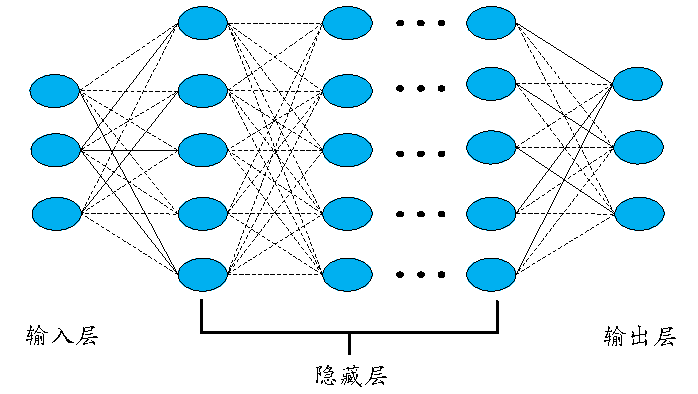
\includegraphics[width=11cm,height=7cm]{深度神经网络结构.pdf}
	%	\centerline{原始样本}
	\setlength{\abovecaptionskip}{5mm} %图片标题与图片距离
	\caption{深度神经网络结构图}
	\label{深度神经网络结构图}
\end {figure}

DNN可以看作是将一组输入变量转化为一组输出变量的非线性数学函数。每个神经元都有对应的权重和偏置参数,控制着输入的精确转化,这些参数在反向传播的过程中,通过损失函数和梯度下降算法来更新。确定这些参数的过程称为DNN模型的学习或者训练,并且需要大量的计算资源,然而权重一旦确定,DNN模型就可以快速的处理相似类型的新数据,识别并提取海量数据中的复杂特征。

以下是本文中涉及到DNN知识产权保护领域中的相关术语:

\begin{enumerate}
	\renewcommand{\labelenumi}{\theenumi)}
	\item 源模型。源模型也称作目标模型,是指模型所有者在私有或公共数据集上,消耗大量计算资源和人力资源训练出的高性能DNN模型,可能因学术研究放置在开源社区,或者作为商用给用户提供远程API。
	\item 可疑模型。可疑模型也称作替代模型,是指该模型可能是通过模型窃取攻击方法从源模型派生出来的模型,判断一个可疑模型是否是从源模型派生是模型知识产权保护领域的主要目标。
	\item 白盒模式。白盒模式是指能够获得DNN模型的所有知识,包括训练集,训练方式,模型参数,模型结构等。
	\item 黑盒模式。黑盒模式指不清楚模型内部参数和结构等,但可以通过模型提供的API获得指定输入的输出。
\end{enumerate}



\section{对抗性攻击}

\subsection{对抗性样本}
 
对抗性样本的概念是Szegedy等人\cite{szegedy2013intriguing}提出的。这篇文章中指出,通常情况下,一个良好性能的DNN模型具备很好的泛化能力,对输入的随机微小扰动具有鲁棒性,因此小扰动不应该改变图像的预测类别。然而,对图像添加特定的非随机扰动,使得损失函数的值增大,可以任意改变DNN模型的预测结果。这种人类肉眼上难以察觉但可以使模型输出错误类别的样本称为对抗性样本。 

用$f:R^m \rightarrow {1,2,...,n}$表示将一张图片映射为$n$个标签的DNN分类器,对一个正常样本$x \in R^m$以及一个错误标签$l$,目标是找到一个最小的扰动$\delta$,使得分类器将样本$x$错误分类为$l$,如式\ref{eq:1}所示:
\begin{equation}
	\label{eq:1}
	\begin{split}
	&min\parallel \delta \parallel_2, \\
	 &s.t. \ f(x + \delta) = l,\ x + \delta \in [0,1]^m
	\end{split}
\end{equation}
其中叠加了扰动的$x +\delta$即为一个对抗性样本。\ref{eq:1}这种方式通常用在黑盒的场景下,仅根据DNN分类器的输出进行扰动$\delta$的调整。
 
 在白盒场景下,由于知道模型的所有知识,可以根据这些信息来寻找对抗性样本,通常利用DNN分类器的损失函数来寻找对抗性样本。
 
 用$f:R^m \rightarrow {1,2,...,n}$表示将一张图片映射为$n$个标签的DNN分类器,对一个正常样本$x \in R^m$以及它对应的正确标签$y$,目标是找到一个足够小小的扰动$\delta:\delta \leq \gamma$,使得加上扰动后的样本输入DNN模型后,损失函数$L$达到最大值,如式\ref{eq:2}所示:
 \begin{equation}
 	\label{eq:2}
 		\delta = arg \mathop{max} \limits_{\delta \leq \gamma} L(f(\theta, x + \delta), y)
\end{equation}
其中$\theta$是分类器$f$的参数,$x + \delta$是一个扰动后的对抗性样本。
 
 \subsection{对抗性攻击的类别}

对抗性攻击技术是指生成对抗性样本的方法,不同的方法生成对抗性样本的效率,质量也不相同。根据方式的不同,可以分为以下几类:

\begin{enumerate}
	\renewcommand{\labelenumi}{\theenumi)}
	\item 白盒攻击与黑盒攻击。白盒攻击指敌手知道DNN模型的参数和内部结构等信息,利用这些信息发起的攻击。黑盒攻击指敌手仅根据模型的输入输出来发起攻击。
	\item 有目标攻击和无目标攻击。有目标攻击指对抗性样本的预测类别为敌手指定的类别,例如将一张牛的图片识别为羊,而不能是其他类别,常采取的方式是向各个方向搜索扰动来最大化DNN模型预测特定类上的可能性。无目标攻击指添加扰动来改变原始预测类别,对具体分类类别不做要求。通常来说有两种攻击方式,一种是最小化DNN模型预测正确类的可能性,一种是进行多次不同类别的的有目标攻击,然后在多个对抗性样本中选取扰动最小的。
	\item 单步攻击和迭代攻击。单步攻击指通过一次添加扰动生成对抗性样本,迭代攻击指通过多次迭代添加微小扰动来生成对抗性样本。通常来说迭代攻击的成功率较高,但是相应的算法复杂度更高,效率较低。
	\item 个体攻击和普适性攻击。个体攻击指针对每个样本都需要重新生成扰动,普适性攻击指找到一个通用的扰动,对数据集中的一类数据都叠加该扰动,普适性攻击效率较高,但是寻找通用扰动的难度较大。
\end{enumerate}

\section{生成对抗网络}

Goodfellow等人\cite{goodfellow2014generative}第一次提出了生成对抗网络(Generative Adversarial Network, GAN),是一种通过生成模型实现无监督学习的特殊方法。GAN由一个生成器和一个判别器构成,训练是一个相互博弈的过程,如图\ref{生成对抗网络结构图}所示,首先随机噪声作为生成器的输入,生成器生成和真实图片维度一致的图像,使用原始图片和生成图片分别输入判定器,训练判定器区分它们的能力,再训练生成器,使之尽可能接近真实图片,通过迭代的交替训练,最终生成器生成的图片和原始图片在空间分布上基本一致,判定器判定生成图片和原始图片为真的概率均为$1/2$,也就是无法区分生成图片和原始图片。

\begin{figure}[htbp]%%图,[htbp]是浮动格式
	\centering
	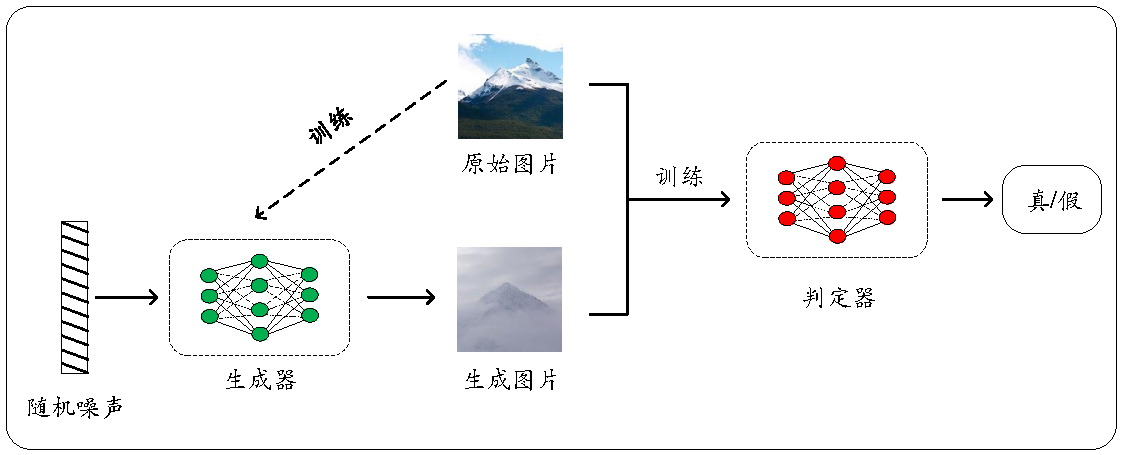
\includegraphics[width=14.5cm,height=7cm]{生成对抗网络结构.pdf}
	%	\centerline{原始样本}
	\setlength{\abovecaptionskip}{5mm} %图片标题与图片距离
	\caption{生成对抗网络结构图}
	\label{生成对抗网络结构图}
\end {figure}

具体而言,生成器$G$和判别器$D$可视为博弈中的双方,当训练GAN模型时,生成器$G$和判别器$D$通过更新各自的参数使损失达到最小,经过不断迭代优化,最后$G$和$D$达到纳什均衡。GAN的目标函数如式\ref{eq:3}所示,对于原始图片$x$,判别器希望$D(x)$变大,对应于式中的$maxD$,对于生成图片$G(T)$,生成器希望$D(G(T))$变大,即$log(1 - D(G(T))$变小,对应于式中的$minG$,所以GAN的目标函数由两个目标构成。
\begin{equation}
	\label{eq:3}
	\begin{split}
		\mathop{min} \limits_{G} \mathop{max} \limits_{D} V(D, G) &= \mathop{min} \limits_{G} \mathop{max} \limits_{D} E_{x \sim P_{data}(x)}[logD(x)] \\
		&+ E_{T \sim P_{T}(T)}[log(1 - D(G(T)))]
	\end{split}
\end{equation}
其中$x$表示原始图片,$T$表示用于生成样本的随机噪声,GAN对噪声$T$的分布没有特别要求,但是常用的有高斯分布,均匀分布,E表示数学期望。

\section{深度神经网络的模型窃取攻击}

自DNN在各个领域取得巨大成功以来,针对DNN模型的攻击就层出不穷,按照攻击方式的不同,可以分为以下三类\cite{xue2021intellectual}:
(1)模型修改攻击。指常见的模型修改,主要包括包括模型微调,模型剪枝,模型压缩,模型再训练等方式。
(2)删除攻击。指攻击者试图逃避水印或指纹的检测,主要包括删除攻击,篡改攻击,逆向工程攻击等方式。
(3)主动攻击。指攻击者主动攻击和强攻击,主要包括歧义攻击,水印和指纹覆盖攻击,查询修改攻击等方式。

\subsection{模型修改攻击}

模型盗窃者在盗窃DNN模型后,通常会对DNN模型进行修改或者压缩,然后部署模型作为MLaas来非法盈利。模型修改主要包括:

\begin{enumerate}
	\renewcommand{\labelenumi}{\theenumi)}
	\item 模型微调。微调通常用于迁移学习中,包括在源模型的基础上,根据自己定制的任务,继续训练模型,使得DNN模型在保持性能的同时修改内部的参数。模型微调可以从源模型派生出非常多的模型。由于内部参数发生改变,水印等可能也会随之变化,因此这对水印的鲁棒性是一个考验。
	\item 模型剪枝。由于DNN模型通常内存占用多,计算开销大,因此模型剪枝是在小型设备上部署DNN模型的常用方法。但是模型盗窃者可能会利用剪枝来删除水印,因此有效的水印技术应该能够抵御由模型剪枝引起的参数变化。
	\item 模型压缩。模型压缩可以显著降低DNN模型的内存需求和计算开销,常用的方法是知识蒸馏,通过将大型模型包含的知识转移到小模型上来达到模型压缩的目的。
	\item 模型再训练\cite{namba2019robust}。模型再训练是一种很直接的方法,这样能尽可能的去除或者减少原有水印的影响,相应的,这种攻击方式成本也比较高。
\end{enumerate}



\subsection{删除攻击}

目前大部分DNN模型的知识产权保护工作专注于水印对DNN模型被修改时的鲁棒性,而很少考虑水印或指纹本身受到的攻击。删除攻击主要包括:

\begin{enumerate}
	\renewcommand{\labelenumi}{\theenumi)}
	\item 删除攻击\cite{shafieinejad2021robustness}。攻击者试图修改模型以删除原有的水印。
	\item 篡改攻击。攻击者知道DNN模型中存在水印,试图窜改模型来删除原有的水印和指纹特征。
	\item 逆向工程攻击\cite{fan2019rethinking}。如果攻击者知道并可以获得原始训练数据,可能会直接对内部参数进行逆向工程。
\end{enumerate}

Shafieinejad等人\cite{shafieinejad2021robustness}研究了DNN中基于后门的水印方法的移除攻击,表明攻击者可以仅依靠公共数据集删除水印,而不用访问训练集和模型参数。还提出了一种检验水印的方法,表明基于后门的水印不够安全,无法保持水印的隐藏。


\subsection{主动攻击}

除了被动的攻击方式,攻击者还可能对DNN模型发动更强的主动攻击。主动攻击主要包括:

\begin{enumerate}
	\renewcommand{\labelenumi}{\theenumi)}
	\item 歧义攻击。歧义攻击指在DNN模型上伪造额外的水印来混淆所有权的验证。研究表明,除非采取不可逆的水印方案,否者即使是鲁棒性的水印,也不一定能验证模型的所有权\cite{fan2019rethinking}。
	\item 水印覆盖攻击\cite{darvish2019deepsigns, chen2019blackmarks, chen2019deepmarks}。即使攻击者不知道具体的私有水印信息,但他知道模型水印嵌入的方法,就可能通过在DNN模型中嵌入新的水印来覆盖原有的水印,从未破坏原有的水印使其不可读。
	\item 查询修改攻击。攻击者修改查询结果来使得水印验证过程无效。一个典型的方式是攻击者获得DNN模型并部署为MLaaS后,会主动检测一个查询是否为水印验证查询,从而修改或者屏蔽该查询,使水印验证无效。
\end{enumerate}


\section{深度神经网络模型的知识产权保护}

训练一个高性能DNN模型需要该领域专家的先验知识来设计模型结构,大量的训练数据和昂贵的计算资源和漫长的训练时间,因此,训练后的DNN模型属于模型所有者的知识产权。得益于DNN模型在各个领域的高效应用,许多不法分子开始偷盗,复制和修改这些模型来提供服务盈利。为了保护DNN模型的知识产权\cite{JFYZ202205002,WXAQ202202001},许多学者受多媒体数字水印的启发,使用模型水印和模型指纹来验证DNN模型知识产权。

\subsection{模型水印}

模型水印是第一种被提出的保护DNN模型知识产权的方法,根据水印嵌入方式和提取方式的不同,主要分为白盒水印和黑盒水印。

在白盒场景下,模型所有者可以利用模型的全部知识构造水印,这些知识包括训练数据集,训练方法,模型内部权重参数和结构。Kuribayashi等人\cite{kuribayashi2020deepwatermark}提出一种基于全连接层权重的可量化水印嵌入方法,通过在训练中改变参数,可以量化水印的影响,从而保证嵌入水印引起的变化较小。不同于基于权重的方法,基于内部结构的水印方法抵抗模型修改的鲁棒性更强。可以在DNN模型中添加一个额外的护照\cite{fan2019rethinking},比如在模型卷积层后面添加一个额外的护照层,以此来作为数字签名,这种方式还可以解决模型受到歧义攻击的问题。

在黑盒场景下,模型所有者不知道可疑模型的内部结构和权重参数等,只能通过API进行访问。一般而言,是通过构造特殊的触发集来实现的,主要有以下几种方式:

\begin{enumerate}
	\renewcommand{\labelenumi}{\theenumi)}
	\item 通过更改样本标签构造触发集,将原始样本标签更改为模型所有者指定的与原始内容不符合的标签,这样仅修改标签不做任何其他修改的水印方法称为零位水印。
	\item 通过在原始样本中嵌入额外水印信息和更改标签构造触发集,这样可以在模型输出中嵌入模型所有者的版权信息。
	\item 通过添加新的样本构造触发集,这样的方式对模型的精度影响较大,一般通过模型微调最大限度的减少新样本对模型决策的影响。
\end{enumerate}


\subsection{模型指纹}

模型指纹一般是利用模型本身来寻找和提取一些固有的特征来作为指纹。相较于模型水印的方法,模型指纹一般不对模型进行修改,因此不会影响模型的精度。一般来说,可以选择靠近决策边界的对抗性样本作为模型的指纹特征,来验证模型所有权。模型指纹分为指纹生成和指纹验证两个阶段。

\noindent\textbf{(1) \ \ 模型指纹生成}

模型指纹与生物学上的指纹类似,具有唯一标识性,用以标记DNN模型的所有权。根据之前对指纹的相关研究\cite{zhao2020afa,lukas2019deep,cao2021ipguard},可以把靠近决策边界的对抗性样本作为模型的指纹。具体来说,通过将此类样本输入DNN模型,将其对应的输出标签作为模型的指纹。

对于一个正常样本$x$,添加一个微小的扰动$\delta$,使得第$i$个输出满足:
\begin{equation}
	\label{eq:4}
	arg \mathop{max} \limits_i g_i(x) = y \wedge arg \mathop{max} \limits_i g_i(x + \delta) = y'
\end{equation}
其中$y$表示输入样本$x$对真实标签,叠加扰动后输出$y' \neq y$,$\delta$是对抗扰动,$x + \delta$即为对抗样本。

所以一组对抗性样本作为指纹样本,对应的输出作为指纹标签,共同构成模型指纹。即$X' = \{x_1',x_2',...,x_n'\}$作为模型指纹样本,对应的预测结果$Y' = \{y_1', y_2',...,y_n'\}$为指纹标签。

\noindent\textbf{(2) \ \ 模型指纹验证}

在模型指纹验证阶段,通常的做法是使用指纹样本查询可疑模型API,比较API返回的预测标签和指纹标签的匹配程度。设定一个阈值$\tau$,当阈值标签和指纹标签的匹配率超过阈值$\tau$时,视为匹配成功。

设$X' = \{x_1',x_2',...,x_n'\}$为$n$个指纹样本,$Y' = \{y_1', y_2',...,y_n'\}$为对应的指纹标签,将$n$个指纹样本输入可疑模型API后,预测标签为$\widetilde{Y}' = \{\widetilde{y_1}', \widetilde{y_2}',...,\widetilde{y_n}'\}$。其中预测标签与指纹标签相同的数量为$q$,即$y_i' = \widetilde{y_i}'(i = 1, 2,...,q)$。

定义验证函数如下:
\begin{equation}
	\label{eq:5}
	Verify(Y', \widetilde{Y}')= \left
	\{ 
	\begin{array}{ll} 
		1, &\quad \dfrac{q}{n} \geq \tau \\ 
		\\
		0, &\quad \mbox{其他}\\ 
	\end{array} 
	\right.
\end{equation}
式\ref{eq:5}中,$q/n$表示匹配成功率,$\tau$是阈值,结果为$1$代表判定可疑模型为盗版模型。


\section{本章小结}

本章主要介绍了深度神经网络,对抗性攻击,生成对抗网络,深度神经网络的模型窃取攻击和知识产权保护这五个方面的相关概念和理论基础。DNN复杂的结构使其训练昂贵耗时,但是一旦训练完成就可以快速处理新数据。对抗性样本是一种人类肉眼无法察觉到变化而会导致模型输出错误的特殊样本,根据方式的不同,有多种产生的方法。生成对抗网络具有强大的特征提取能力,可以利用其生成类似训练样本特征分布的新样本。根据攻击强弱的不同,可以将DNN模型窃取攻击分为模型修改攻击,删除攻击和主动攻击。在DNN模型知识产权保护领域,目前使用最广泛的是模型水印和指纹这两种方法。
